% CREATED BY MAGNUS GUSTAVER, 2020
\chapter{Theory} \label{Theory}
This section presents theory used in this thesis. It starts with the hardware used to
enable autonomous flight of the drone, then the software and how communication between the computer the phone is handled. 


\todo{Se till att theory INTE innehåller någofn form av implementation, det som står i theory ska presentera den hård- och mjukvara som vi får tilldelat samt deras begränsingar}



\section{Hardware} \label{Hardware}
In this section the hardware that is used will be presented, which is a drone, a mobile device and the test objects. 

\subsection{DJI mavic 2 enterprise zoom} \label{DJI}


\begin{figure}[h!]
\centering
 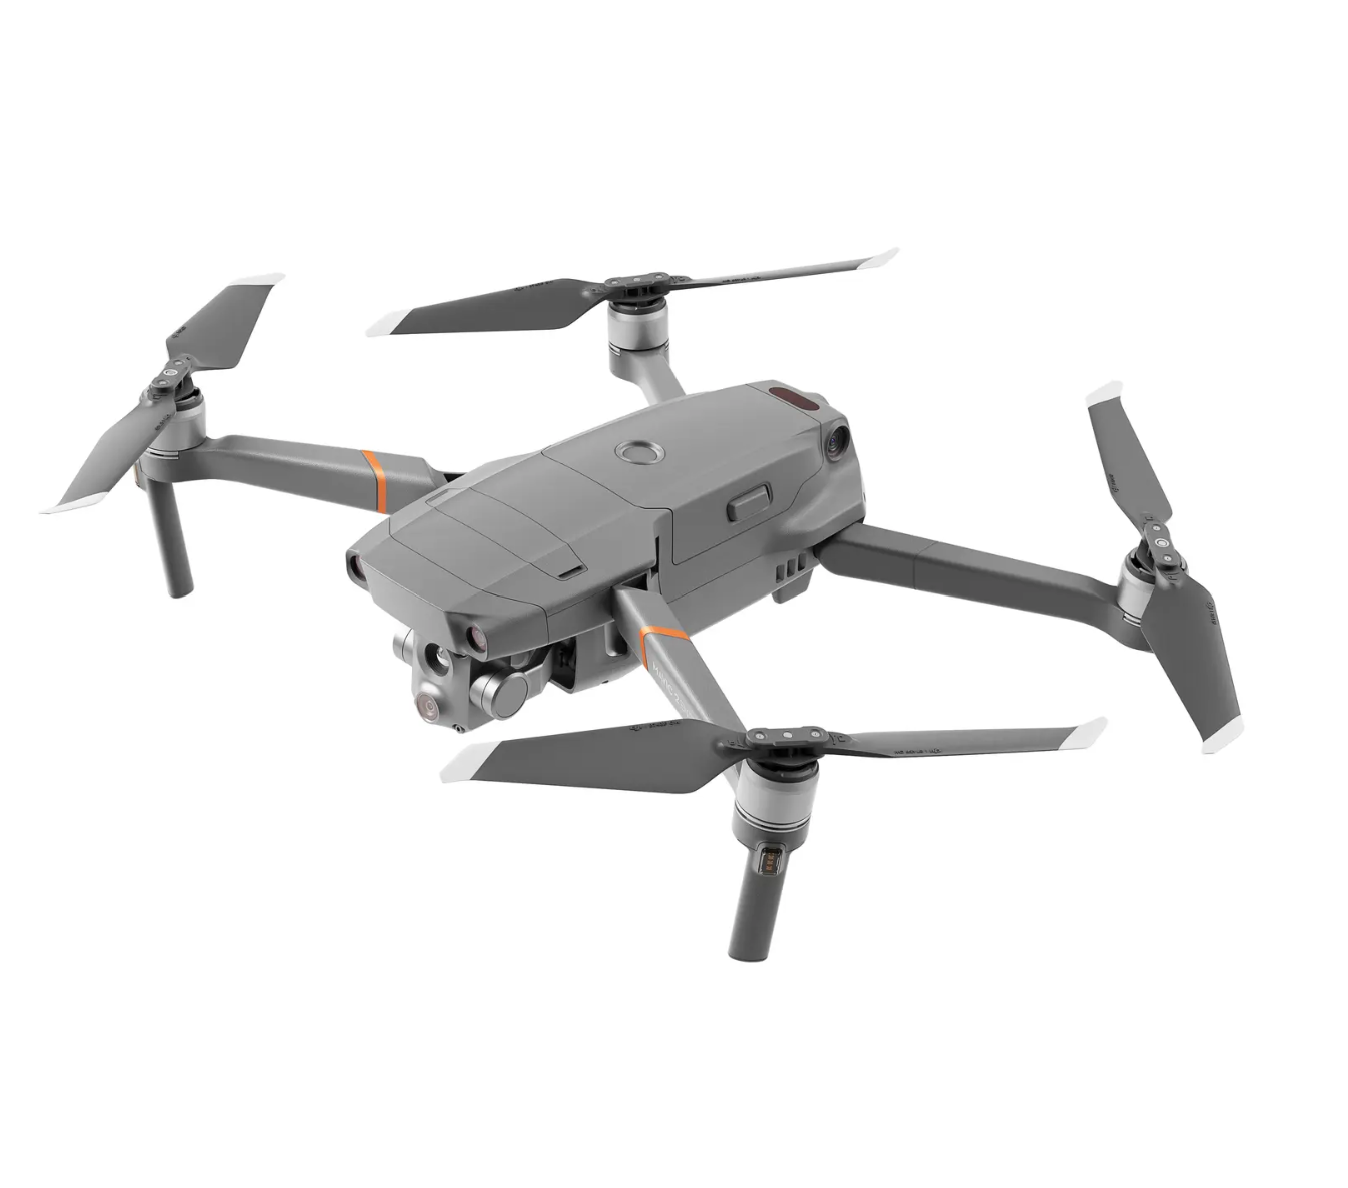
\includegraphics[width=0.65\textwidth,angle =0]{figure/DJI_mavick_2_enterprise.png}
\caption{Picture of the DJI Mavic 2 Enterprise ~\cite{DJI2021MAVICMANUAL}}
\end{figure}


The unmanned aerial vehicle (UAV) utilized in this project is the DJI Mavic 2 Enterprise, developed by the Chinese technology company DJI. This UAV has garnered widespread popularity in the commercial and industrial community due to its compact design, advanced camera capabilities, and ease of use.
\newline

The Mavic 2 Enterprise is equipped with a 3-axis gimbal stabilized camera that can capture high-quality 4K video and 12MP photos ~\cite{DJI2018MavicDJI}  . It features omnidirectional obstacle sensing and avoidance with sensors positioned on the front, back, bottom, and sides, as well as a GPS and magnetometer sensor, which allows the drone to maintain a stable hovering position.
\newline

%\textcolor{red}{Ska detta vara med? In order to control the drone, an RC is necessary, which communicates with the drone on 2.4GHz or 5.8GHz depending on the surroundings.}
A compatible smartphone with a designated application must be connected to the RC via an USB cable if a live feed from the drone is desired. DJI offers its own application that offers pilots a wide array of modes, settings, and options to customize and monitor the live feed from the drone. This application can be downloaded from either the App Store or Google Play. However, given the autonomous nature of this project, a bespoke application tailored specifically for this purpose had to be developed.
\newline 

The Mavic 2 Enterprise has a maximum flight time of up to 31 minutes and a range of up to 8 kilometers, making it a versatile and effective tool for various applications. However, it is important to note that drone laws and regulations vary by country and region, and certain areas may require permits to fly beyond visual line of sight or certain distances. Therefore, strict adherence to local regulations and safety protocols is of paramount importance when operating the Mavic 2 Enterprise or any other UAV.



\subsection{Samsung A13} \label{Samsung}
\begin{figure}[h!]
\centering
 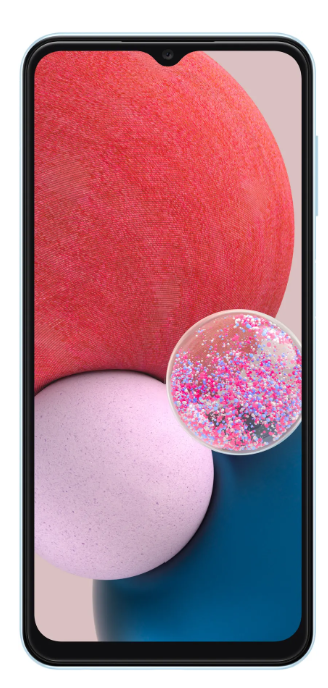
\includegraphics[width=0.25\textwidth,angle =90]{figure/Samsung_A13.png}
\caption{Picture of the Samsung A13}
\end{figure}
The device Samsung Galaxy A13 is an affordable and reliable mobile device with a long-lasting 5,000mAh battery.
In summary, the Samsung Galaxy A13 is a cost-effective and reliable mobile device that offers users a range of features and capabilities. Its robust hardware and user-friendly software make it a suitable choice for various applications, from basic computing tasks to multimedia editing and communication.



\section{Software} \label{Software}
This section will describe the software that is being used in this project, which is DJI Mobile SDK, ATOS, Android and Java.


\subsection{ISO DTS 22133 Communications Protocol} \label{ISO}
\todo{Skriva om skriva rätt //MS}
In order to properly test collision avoidance systems and carry out numerous other test, it is necessary to conduct testing on the specialized proving grounds, a controlled environment that is safe for both the driver and other motorists. In order to create realistic traffic scenarios, the proving grounds must make use of various targets that can represent both vehicles and / or pedestrians.

The ISO DTS 22133 document states the requirements, functionality, and protocol necessary for controlling multi target-carrier systems to create and monitor realistic traffic scenarios in a safe and effective manner. The ISO22133 is a standard designed to work with multiple manufacturers and different objects. Each object holds a state which is controlled from the control center. 
\\ \\
\begin{figure}[H]
  \centering
  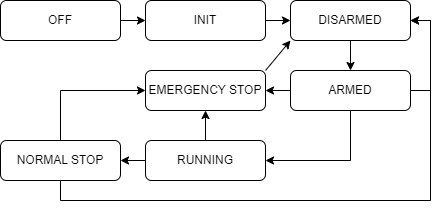
\includegraphics[scale=0.6]{figure/ISO-states.png}
  \caption{Illustration of relevant object states and their transitions}
  \label{fig:iso_states}
\end{figure}
Figure~\ref{fig:iso_states} displays the various states and transitions of the test object, each representing a specific action. In the ''Init'' state, the object is initialized but not connected to the control center. When the control center establishes a successful connection, the object moves to the ''Disarmed'' state, meaning it's ready to receive telemetry data and begin mission planning. Once armed, the object receives the telemetry data and is set to execute the test. During the ''Running'' state, all objects follow their predetermined trajectories until each object reaches its endpoint. The test then moves to the ''Normal Stop'' state, indicating that the test has concluded. From ''Normal Stop,'' the objects can transition back to the ''Disarmed'' state to repeat the sequence. Additionally, the ''Disarmed'' state can be reached from the ''Emergency Stop'' state, which acts as a kill switch to abort the test.
\\ \\
Note that some states from the ISO22133 protocol are not shown in the figure, as they're not relevant to this project. One such state is the ''Remote Ctr'' state, which allows the operator to move the object freely without relying on predetermined telemetry, while still maintaining a connection to the control center.
\subsection{Autonomous Vehicle testing operating system (ATOS)} \label{ATOS}
The core of each test is ATOS, short for Automatic Vehicle Testing Operating System, which follows the standards stated in the ISO22133 documentation and creates trajectories for each object that is part of the test. An extensive comprehension of the ATOS software needs to be obtained, this includes the functional requirements, software specifications and the communication protocol. The information can be obtained from the ISO22133 protocol \todo{\cite{} till ISO} as well as in the actual codebase \cite{AstaZero2023ATOS:Systems.}. The project is mainly written in the programming languages C and C++ and developed on and Linux platform. The integration of ATOS in this project is illustrated in Figure~\ref{fig:ATOS-flow}.
\begin{figure}[H]
  \centering
  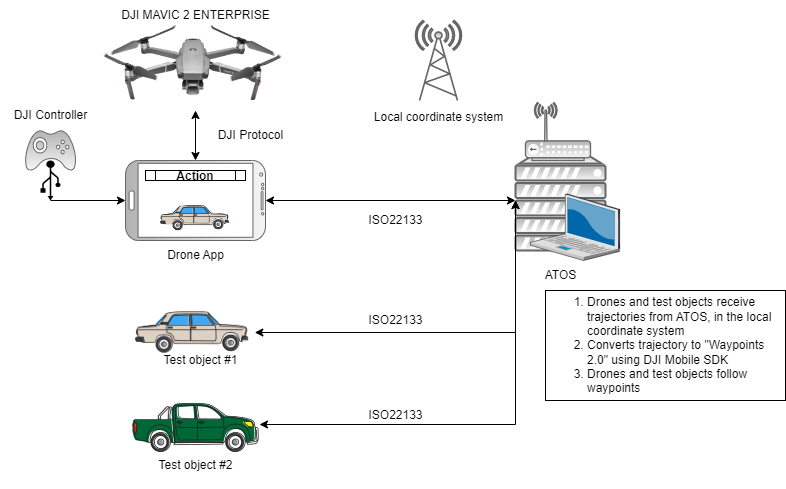
\includegraphics[width=\columnwidth]{figure/flow_config.png}
  \caption{ATOS integration with other objects}
  \label{fig:ATOS-flow}
\end{figure}




\subsection{Linux and Ubuntu 20.04} \label{Linux}
As stated in the last section, ATOS is being developed using a Linux operating system, specifically Ubuntu 20.04. Linux and Windows have some fundamental differences making it impossible to compile projects aimed at Linux operating systems on Windows. Both the ATOS project and the Android application provided by AstaZero have dependencies on other Linux programs which is why an old version of the Ubuntu operating system was required. The team therefore had to familiarize themselves with Ubuntu 20.04 and use it for all development purposes during the project. 

\subsection{Java, Android, SDKs and Android Studio} \label{Java, Android....}
The application is programmed in one of the major mobile operating systems named Android \todo{Ska de bara vara fakta här eller kan man skriva såhär?}. Android provides a framework for communicating with any mobile device running the Android operating system. The operating system is built using different activities which represent different parts of the application \todo{referens} and focuses on one single thing a user can do \cite{Android}. For instance, one activity could be the landing page of the application while another activity could be the interface which communicates with the drone. Together these different activities makes up the application and communicate which each other.
\\ \\
The recommended option to develop Android applications is Android's own program called Android Studio. The program provides all necessary tools for developing Android applications in Java. It has also support for designing the user interface in both a visual studio and using the programming language XML.
\\ \\
Android enables the developers to use outside libraries, also called Software Development Kits (SDK). These external libraries allows the developer to use other code written by other developers and use their frameworks. DJI provides their own SDK for communicating with their different products.
\newline
To access the functionalities of the DJI Mavic 2 Enterprise drone, a mobile application must be connected to the drone's remote controller (RC). As previously stated, DJI provides a framework for Android devices, which enables users to access functions such as reading drone states, initiating or terminating video recording, obtaining a live feed from the drone's camera, land at a given point and starting or stopping the motors. DJI's website contains tutorials on how to implement various types of functions for the application, which have served as a foundation for learning how to communicate with the drone in this study. Moreover, GitHub hosts a diverse range of projects of varying kinds that have been explored to acquire knowledge of the DJI Mobile SDK API.
Given that AstaZero provided an Android phone, the app development was limited to Android.


\subsection{AstaZero's application} \label{AZ's app}
\todo{SKRIV. Axel gör detta /Teddy, kort o koncist}
\subsection{DJI WaypointMission}
\todo{SKRIV}
The drone is able to fly on it's own with different protocols provided by the DJI SDK. One of these protocols is the WaypointMission \cite{WaypointMission}\todo{ref funkar inte} which enables the developer to create a list of geographical locations to which the drone will fly. The developer is able to control the speed, heading, latitude and longitude the drone should have at each waypoint. It also offers a callback for different events such as mission start, waypoint reached and mission uploaded. This can be utilized to perform different actions based on the state of the mission.  
\todo{Vetefan vad mer man kan skriva här //MS}
\subsection{Object detection} \label{Image tracking}
In order to ensure that the camera capture the vehicles at the optimal angle, it was imperative for the drones to accurately detect the location of the cars as the drones followed them.  
\\ \\
Image recognition is a rapidly developing field of computer vision that has gained significant attention in recent years. At its core, image recognition involves the automatic identification and classification of objects within digital images. This is accomplished through the use of sophisticated algorithms, which are designed to recognize specific patterns and features within the image data.
\\ \\
According to Myeongsuk and Sanghoon in their paper ''A review of deep learning in image recognition'', published in the Institute of Electrical and electronics engineers (IEEE) \cite{Pak2018ARecognition}, the process of image recognition is typically achieved using deep learning algorithms, such as convolutional neural networks (CNNs). These networks consist of several layers, including convolutional, pooling, and fully connected layers, which work together to extract and analyze features from the input image.
\todo{Fråga till Martin Fabian: Räcker detta eller ska man förklara vad t.ex. convolutional, pooling och fully connected är?}
\\ \\
TensorFlow Lite is a library specifically developed for mobile applications which offer pre-trained models for different scenarios. One scenario is object detection. Since a phone does not have the same processing power as a normal computer the Lite models are a compressed version of the normal TensorFlow models and are less sophisticated compared to normal models. In other words, a TensorFlow lite model trades a bit of accuracy for a great increase in computational speed compared to a normal TensorFlow model, which fits our task of running such a model on a phone. 
\\ \\
The team made the decision to find and implement an existing pre-trained object detection model. While parts of the team had image classification experience, where convolutional layers were combined with a neural network to form a CNN, the task of classifying a single class from an image with the object in it's center is vastly different from object detection. In object detection, there is no certainty that the desired object is in the center of the image and there can be multiple objects present in the same image. Creating a model which could handle this and then training said model seemed too time-consuming since research in the field has produced efficient and accurate pre-trained models.
\\ \\
The problem of classifying \todo{fixa källor} multiple different objects with varying positions in an image has many solutions. Deep learning, specifically neural networks became the state of the art method for object detection in 2014 with the development of R-CNN:s (Regions with Convolutional Neural Networks). These networks showed great improvements in accuracy but were rather slow and computationally expensive, not suitable for real-time object detection. In R-CNN an algorithm called selective search is used on the image, which solves the problem of detecting multiple objects with varying size and position in various images. This algorithm proposes regions of an image likely to contain an object. The proposed regions are then sent as inputs to a CNN which in turn outputs data to a SVM. The SVM receives features extracted by the CNN, which it uses to classify the region. 
\\ \\
Since then, improvements have been made. Single-shot Multibox Detection (SSD) is one of those improvements. It uses the convolutional layers of some image classification model to produce detailed feature maps. A feature map is the result of applying a convolutional layer to an image. Convolutional layers use a filter of a certain size to detect features in an image. The lower (or earlier) convolutional layers identify simple features such as edges and the more convolutional layers and filters added, the more complex the identified features can be. These feature maps are then sent to the head of the SSD.

\subsection{Tracking Algorithm} \label{Tracking algorithm}

Object detection is a crucial process for identifying specific objects within an image or video frame. However, object tracking takes this process to the next level by not only identifying the objects, but also monitoring their movement over time.
\\ \\
To facilitate this transition, one of the most widely-used approaches is implementing an algorithm that can trace the identified objects from frame to frame. This is achieved by employing a tracking algorithm that utilizes a combination of features such as color, texture, and shape to effectively monitor the objects \todo{ref till Pengfei Zhang, Wei Zhu, and Hailin Jin. (2020). Object Detection and Tracking: A Review. IEEE Transactions on Intelligent Transportation Systems, 21(12), 5101-5119. doi: 10.1109/TITS.2019.2958714. IEEE xplore ligger nere}.
\\ \\
Several algorithms have been proposed for object tracking, including the Kalman filter, which utilizes a mathematical model to anticipate the object's position in the next frame based on its previous location and velocity. Additionally, deep learning-based tracking techniques, such as Siamese networks or correlation filters, can be employed to learn how to track objects based on their appearance characteristics. Once the objects are successfully tracked, the system can predict their location in future frames, resulting in better tracking and movement prediction.

\subsection{Graphical User Interface} \label{GUI}
Developing the GUI for the app includes designing an effective, functional and informative interface that is easy to use while also providing all the necessary controls for operating it and capturing the footage. Below are some scientifically based ~\cite{AntchevaGUIDELINESGUI}, as well as some project-based, considerations for GUI-development. 
\\

\begin{itemize}
    \item \textbf{Creating a user centered interface:} The GUI should be intuitive and easy to navigate. 
    \item \textbf{Include all necessary commands:} Evaluate what commands are needed for executing the program and make them easily accessible. 
    \item \textbf{Create a distinct visual hierarchy:} Prioritize important information and make it easy for the user to locate the necessary information. 
    \item \textbf{Real-time representation:} The GUI should provide users with the real-time footage captured by the drone as well as real time updates of the drones battery life etc. 
    
\end{itemize}


%% GUIDELINES FOR DEVELOPING A GOOD GUI,https://indico.cern.ch/event/0/contributions/1294438/attachments/747/1334/IA_CHEP04_paper.pdf








%\section{Equation}
%\begin{equation}
%f(t)=\left\{ \begin{array}{ll}
%1,~~~~ & t< 1 \\
%t^2 & t\geq 1
%\end{array}\right.
%\end{equation}

%\section{Table}
%\begin{table}[H]
%\centering
%\caption{Values of $f(t)$ for $t=0,1,\dots 5$.}
%\begin{tabular}{l|llllll} \hline\hline
%$t$ & 0 & 1 & 2 & 3 & 4 & 5 \\ \hline
%$f(t)$ & 1 & 1 & 4 & 9 & 16 & 25 \\ \hline\hline
%\end{tabular}
%\end{table}


%\section{List}
%\begin{enumerate}
%  \item The first item
%  \begin{enumerate}
%    \item Nested item 1
%    \item Nested item 2
%  \end{enumerate}
%  \item The second item
%  \item The third item 
%  \item \dots
%\end{enumerate}

\section{Limitations} \label{Limitations}
This section will delineate the limitations associated with the utilization of the drone hardware, the DJI SDK application with heavy focus in the WaypointMission software as well as the already existing code base. 

\subsection{Hardware} \label{Dron limitations}
Research into the limitations of the drone presented in section \ref{DJI} was needed to obtain necessary information on the feasibility of achieving the performance requirements. The physical limitations does not hinder the project potential as much as the software limitations described in section \ref{limits of dji sdk}. This assumption is purely based on the fact that Euro NCAP tests chosen for this project does not create an environment that pushes the limits of the drone capabilities from a hardware standpoint. Even though the drone hardware limitations, for this specific test does not become a problem, it is worth noting that there exists, for example Euro NCAP tests \cite{speed_euro_ncap} with speeds that exceeds the speed capability of the drone \cite{DJI2021MAVICSERIES}.
\newline 

In addition, the computing power of the Samsung A13 phone presented in section \ref{Samsung} is significantly limited in terms of performance compared to a desktop or laptop computer. This limitation becomes evident when performing tasks that require significant computational power, such as object detection and image recognition algorithms. Despite these limitations, with an appropriately streamlined software, the Samsung A13 can still provide a sufficient level of computational power for on-the-go image recognition tasks, such as identifying cars or people which will be done during Euro NCAP test documentation.


\subsection{Software Development Kit} \label{limits of dji sdk}
DJI offers a commercially available off-the-shelf way to both be able to track objects and follow them at the same time. However, the drone is not capable of running these software packages in parallel, making the built in object detection and tracking useless. This is because the implementation of the WaypointMission software is prioritized, as it facilitates the drone to easily follow predetermined paths as well as enabling maneuvering of the drone camera gimbal in parallel.  
\newline
\label{sec:limit_WP}

The WaypointMission software employed for flying pre-determined missions has certain constraints that limit the drone's range, restricting its flight radius to 500m or less \cite{WaypointMission}. This is likely a safety precaution considering that the remote controller for the drone can operate within a range of around 10km under ideal circumstances. The software's current target tests are aimed at filming within a radius of less than 500 meters, which poses no issue. However, if AstaZero intends to employ the software for conducting tests at ranges greater than this, it must be taken into account to ensure the test's feasibility.
\newline

In addition, WaypointMission has a maximum limit of 99 predetermined waypoints per mission which poses a significant constraint on the drone's accuracy for larger missions and requires attention in the code. The trajectory provided by ATOS may consist of more than 99 points and must be reduced accordingly. See section \ref{sec:alt_douglas_peucker_algo}. 
\newline

The WaypointMissions are predetermined, static and needs to be uploaded to the drone before the test commences. During the test no changes to heading, speed or position can be changed automatically, only manually. This disables the use of a systems control implementation for compensating for wind and / or similar interference. The WaypointMission class offers a way to focus the gimbal on different points of interest at each waypoint. However, since information about where the car is located is not given through the ISO DTS 22133 protocol, this is not an option.


\subsection{Existing code base}
When choosing another algorithm to use for object tracking, it needs to be considered that the provided application by AstaZero is using an older Android SDK version. Most modern object detection algorithms and SDK:s require newer versions of the SDK which greatly limits the options available for performing object detection and tracking.
\todo{Den här är svår att skriva teoretisk //MS}


%\section{To-do note}
%The \texttt{todo} package enables to-do notes to be added in the page margin. This can be a very convenient way of making notes in the document during the process of writing. All notes can be hidden by using the option \emph{disable} when loading the package in the settings. \todo{Example of a to-do note.}

